\section{Durchführung}
\label{sec:Durchführung}
\subsection{Untersuchung des Acrylblocks}
Zunächst wird der zu untersuchende Acrylblock mit einer Schieblehre vermessen. Der verwendete Block ist in Abb. \ref{fig:Block} skizziert, welcher sich auch die Benennung der Fehlstellen entnehmen lassen. Die Fehlstellen sind hierbei als Bohrungen ausgeführt.

\begin{figure}
  \centering
  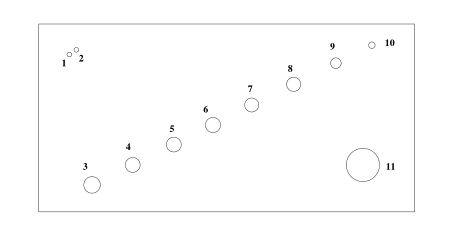
\includegraphics[height = 5cm]{./Block.PNG}
  \caption{Schematische Darstellung des verwendeten Acrylblocks und Benennung der Fehlstellen. \cite{Anleitung}}
  \label{fig:Block}
\end{figure}

\subsubsection{A-Scan}
Die im Block befindlichen Fehlstellen werden durch eine Ultraschalluntersuchung mit einer $\SI{1}{\mega\hertz}$ Sonde die Lagen der Löcher im Block bestimmt, indem der Block einmal "von oben" und einmal "von unten" vermessen wird. "Von oben" Bedeutet hierbei wie in Abb. \ref{fig:Block} dargestellt, "von unten" um $\SI{180}{\degree}$ gedreht.
Um eine bessere Auflösung der Fehlstellen 1 und 2 zu erreichen, wird die Messung mit einer $\SI{4}{\mega\hertz}$ Sonde wiederholt.

\subsubsection{B-Scan}
Erneut werden die Lagen und Größen der Fehlstellen mit Hilfe eines B-Scans bestimmt, bei dem die Sonde von Hand über den Acrylblock gezogen wird.

\subsection{Untersuchung des Herzmodells}
In diesem Versuchsteil wird ein Herzmodell untersucht, welches aus einem Zylinder besteht, welcher durch eine Membran in zwei Berreiche geteilt ist. Der untere Berreich ist luftdicht an einen Gummipumpball angeschlossen, über den sich der Druck im Herzmodell erhöht und somit die Membran aus der Ruhelage auslenkt.
Besagte Membran ist aus \LaTeX gefertigt und bildet unter Normaldruck eine horizontalliegende Ebene. Da sie sehr dünn und elastisch ist, dehnt sie sich bei erhöhtem Druck leicht aus und vergrößert somit das von ihr begrenzte Volumen.
Zur Messung wird die Membran ca. $\SI{2}{\centi\meter}$ hoch mit Wasser bedeckt, auf dem eine Ultraschallsonde aufliegt. Diese kann über einen Time-Motion-Scan die Lage der Membran erfassen.
